% !TeX root = ../main.tex

\chapter{A Fully-Convolutional LSTM Encoder-Predictor Model} \label{chapter:implementation}

This chapter presents the final model that is used in this thesis for future frame prediction. It combines the insights and strengths of previous works that have been analyzed in the preceding chapter. Each component of it is investigeted in detail and then assembled to end up with the overall network architecture. But beforehand, two cruical techniques are presented which improve the learning of spatio-temporal features and the recurrent training performance.

\section{Techniques}

In this section, two important methods are presented that enable recurrent network based models to reach better performance in a shorter time of training. The next section then uses these techniques as building blocks while describing the network architecture.

\subsection{Convolutional LSTM} \label{sec:conv_lstm}

As discussed in earlier chapters, the standard LSTM cell has the drawback of lacking spatial correlations in the input-to-hidden and hidden-to-hidden transitions, because it operates over sequences of vectors with only one dimension. The LSTM activations are computed based on linear transformations using fully-connected layers and subsequent non-linearities. The authors of \parencite{conv_lstm_nowcasting} propose a variant of the LSTM cell with the core idea to handle all inputs, hidden states, cell or gate outputs as 3D tensors to preserve the spatial data properties. This is realized by exchanging the internal matrix products by convolution operations. The resulting recurrent cell type is called \textit{convolutional LSTM} (ConvLSTM).

In contrast to the realization in \parencite{spat_temp_video_autoenc}, peephole connections are included in our implementation of ConvLSTM. These allow the gated units to have a direct access to the previous memory cell state. In addition, we enable it to use optional batch normalization layers in both input-to-hidden and hidden-to-hidden transitions to allow faster learning and to take advantage of its other benefits which have been described in section \ref{sec:batch_norm}. The same modifications have been proposed for the standard LSTM cells in \parencite{rnn-batchnorm}. All this together can be formulated as:

%TODO maybe correct this formula, since we used conv2d instad of hadamard for peepholes as well.
\begin{equation} \label{eq:convlstm}
\begin{aligned}
\Spvek{\tilde{\textbf{f}}^{(\tau)}; \tilde{\textbf{i}}^{(\tau)}; \tilde{\textbf{o}}^{(\tau)}} &= \texttt{BN}(\textbf{W}_{h} \ast \textbf{h}^{(\tau-1)}; \gamma_h, \beta_h) + \texttt{BN}(\textbf{W}_{x} \ast \textbf{x}^{(\tau)}; \gamma_x, \beta_x) + \textbf{W}_{peep} \odot \textbf{C}^{(\tau-1)} + \textbf{b} \\
\hat{\textbf{c}}^{(\tau)} &= tanh(\texttt{BN}(\textbf{W}_{hc} \ast \textbf{h}^{(\tau-1)}; \gamma_h, \beta_h) + \texttt{BN}(\textbf{W}_{xc} \ast \textbf{x}^{(\tau)}; \gamma_x, \beta_x) + \textbf{b}_c) \\
\textbf{C}^{(\tau)} &= \sigma(\tilde{\textbf{f}}^{(\tau)}) \odot \textbf{C}^{(\tau-1)} + \sigma(\tilde{\textbf{i}}^{(\tau)}) \odot \hat{\textbf{c}}^{(\tau)} \\
\textbf{h}^{(\tau)} &= \sigma(\tilde{\textbf{o}}^{(\tau)}) \odot tanh(\texttt{BN}(\textbf{C}^{(\tau)}; \gamma_c, \beta_c))
\end{aligned}
\end{equation}

where $ \textbf{W}_h \in \mathbb{R}^{d_h \times 3d_h} $ and $ \textbf{W}_{hc} \in \mathbb{R}^{d_h \times d_h} $ are the shared weights for the hidden-to-hidden transitions at time step $ \tau $, $ \textbf{W}_x \in \mathbb{R}^{d_x \times 3d_h} $ and $ \textbf{W}_{xc} \in \mathbb{R}^{d_x \times d_h} $ the shared weights for the input-to-hidden connections, as well as $ \textbf{W}_{peep} \in \mathbb{R}^{d_x \times 3d_h} $ the shared weights for the peephole connections. Next, $ \textbf{b} \in \mathbb{R}^{3d_h} $ and $ \textbf{b}_c \in \mathbb{R}^{d_h} $ are the biases, $ \textbf{C}^{(0)}, \textbf{h}^{(0)} \in \mathbb{R}^{4d_h} $ the initial states of the memory cell and the hidden state, respectively. Furthermore, $\ast$ denotes the convolution operation and $ \texttt{BN}(\textbf{x}; \gamma, \beta) $ a batch normalization layer with its learned shift $\gamma$ and scale $\beta$. As in \parencite{rnn-batchnorm}, $\beta_h$ and $\beta_x$ are set to zero by default to avoid the unnecessary redundancy with the existing bias terms $\textbf{b}$ and $\textbf{b}_c$. The structure of such a cell is visualized in Figure \ref{fig:convlstm-cell}.

\begin{figure}[htpb]
	\centering
	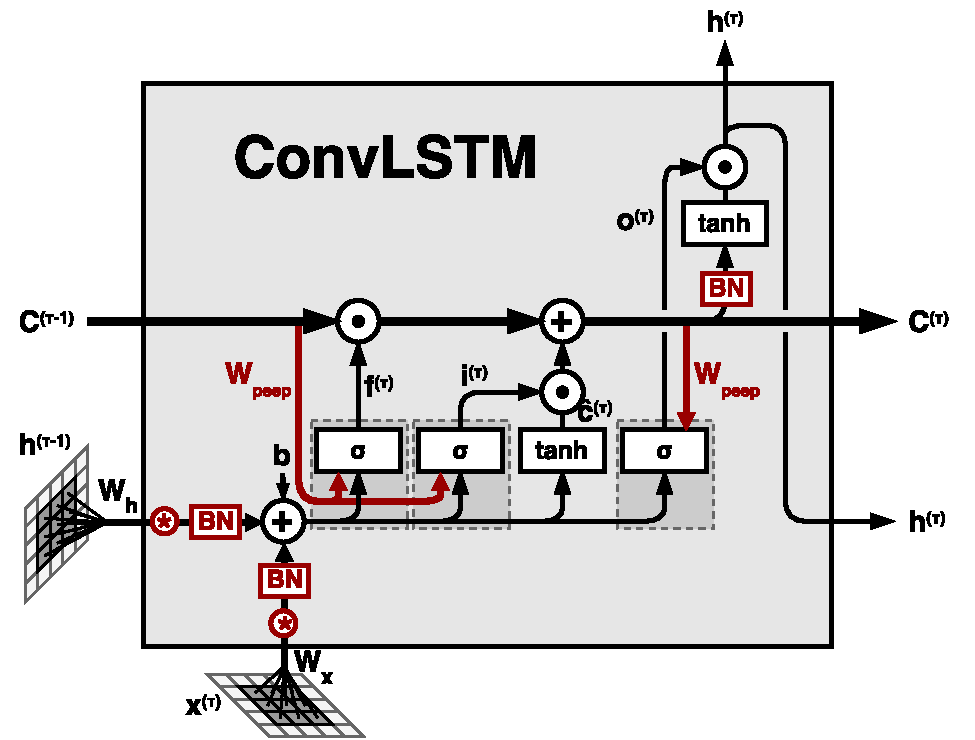
\includegraphics[width=0.65\linewidth]{figures/convlstm.pdf} 
	\caption[ConvLSTM Cell]{The simplified structure of the batch-normalized ConvLSTM cell including peephole connections. The inputs and previous hidden states are convolved to produce 3D tensors that flow through each cell. Changes to standard FC-LSTM are highlighted in red.} \label{fig:convlstm-cell}
\end{figure}


\subsection{Scheduled Sampling} \label{sec:sched_sample}

When the first recurrent network based models have been tested in the course of this thesis, a discrepancy between training and inference has been discovered. At training time, each cell is usually fed with the ground truth $\textbf{x}^{(\tau-1)}$ of the previous time step in order to generate the current prediction $\hat{\textbf{x}}^{(\tau)}$. In contrast, the generated frame $ \hat{\textbf{x}}^{(\tau-1)}$ of the previous cell is used instead as cell input during inference, because no ground truth is available in that case. Thus, mistakes made earlier in the sequence flow through all following cells and can quickly amplify since the network has never dealt with such errors at training time. In context of future frame generation, this effect has been identified when the prediction quality has dropped tremendously after the first generated frame. The fact that predicted frames usually look slightly blurry is the clear reason for this, because a network that was fed purely with ground truth input images has never seen such pictures with smooth edges.

As a first step, the recurrent cell input during the training process has therefore been adapted to behave in the same way as in inference mode. Therefore, a recurrent cell that is trained to generate a future frame has to condition on the previously generated frame instead of the ground truth\footnote{Always conditioning on the generated outputs while training is called \textit{always sampling} (AS) according to \parencite{sched_sample}.}. This strategy can be seen as an automatic form of data augmentation or a natural regularizer and helps the network to learn a robustness against imperfect inputs. However, this comes with the downside that the RNN model converges much slower during the training, because it has to predict the correct output given poor or even wrong input data.

To combine the best of both worlds, we have experimented with a training strategy where each recurrent cell started to condition on the ground truth frame and have slowly changed to the inference mode conditioning using a probability variable $p$ with linear or exponential decay. In this process, a random number $r \in [0, 1]$ is generated at each training step and the RNN cells condition on the generated frame when $r \geq p$. First experiments have shown positive results, because a better performance could be reached compared to both other strategies mentioned earlier. 

Shortly afterwards, we came across \parencite{sched_sample} where the authors propose a similar but even more radical strategy and demonstrate insightful evaluation results. Their so-called \textit{scheduled sampling} (SS) training strategy for recurrent networks is based on the same core idea, but instead of generating only a single random number $r$ for the whole input sequence, they propose to do this for every single time step $\tau$. In addition, they suggest to use an inverse sigmoid decay function in order to provide a smooth transition from training mode to inference mode:

\begin{equation} \label{eq:inverse-sigmoid}
\sigma_{inv}(i; \alpha) = \frac{\alpha}{\alpha + exp(i / \alpha)} ,
\end{equation}

where $i$ identifies the current training step and $\alpha \geq 1$ controls the expected speed of convergence. This function and a diagram of the scheduled sampling approach is depicted in Figure \ref{fig:sched-sample}.

\begin{figure}[htpb]
\centering
\begin{subfigure}{0.5\textwidth}
  \centering
  \hspace*{-0.6cm}
  {
  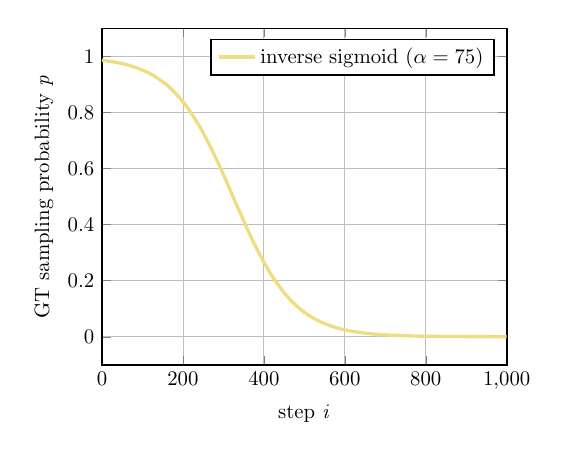
\begin{tikzpicture}[scale=0.75]
    \begin{axis}[
        ymin=-0.1,
        ymax=1.1,
        xmin=0,
        xmax=1000,
        legend style={legend pos=north east},
        grid,
        thick,
        ylabel=GT sampling probability \textit{p},
        xlabel=step \textit{i},
      ]
      \addplot [mark=none,draw=LightGoldenrod,smooth,ultra thick,domain=0:1000] {75/(75+exp(\x / 75))};
      \addlegendentry{inverse sigmoid ($\alpha = 75$)};
    \end{axis}
  \end{tikzpicture}
  }
  \caption{}
  \label{fig:sched-sample-inv-sig}
\end{subfigure}%
\begin{subfigure}{0.5\textwidth}
  \centering
  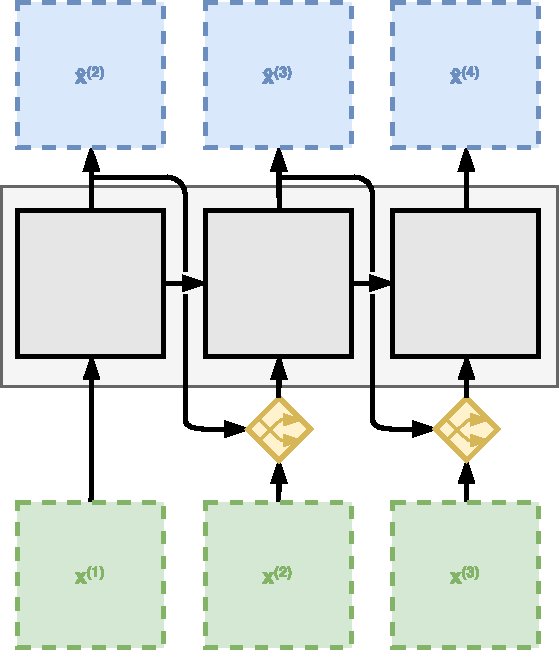
\includegraphics[width=.7\linewidth]{figures/sched_sample.pdf}
  \caption{}
  \label{fig:sched-sample-process}
\end{subfigure}
\caption[Scheduled Sampling]{Illustration of scheduled sampling, where (a) shows the inverse sigmoid decay function and (b) the structure of a RNN that uses this approach. The yellow blocks symbolize the scheduled sampling components, which decide whether a cell conditions on the ground truth or the previous output by flipping an unbiased coin.} \label{fig:sched-sample}
\end{figure}




\section{Network Architecture}

The final model architecture is based on the RNN encoder-decoder framework introduced in Section \ref{sec:rnn_enc_dec} and both previously presented advancements to improve the learning of spatio-temporal features in video data. This architecture has been chosen because it explicitly models the temporal correlations and is flexible regarding the input and output sequence. Further, previous works demonstrated in Chapter \ref{chapter:relatedwork} have shown promising results using this recurrent framework. The architecture that is presented in this section describes the default version of the network that is used for frame prediction of generated image sequences of animated, handwritten numbers. The following evaluation in Chapter \ref{chapter:evaluation} assesses this model with different settings, such as variations in the network's depth.

\subsection{Components} \label{sec:impl-components}

Before the entire network model is demonstrated, we would like to go through its main components in detail first. These components for encoding or decoding are ordered according to the flow of data while propagating forward through the network. Afterwards, the loss layer is presented which combines standard error functions with perceptual motivated bias terms.

\subsubsection{Spatial Encoder}

Instead of feeding the recurrent encoder directly with raw image data like in \parencite{unsup_learn_lstm} or \parencite{conv_lstm_nowcasting}, each frame flows through a multilayer CNN first. Therefore, it is projected to an image percept in feature space of lower size, but higher depth. This single convolutional network is shared across the entire time domain of the spatio-temporal encoder component described next. The motivation to use this spatial encoder is based on \parencite{spat_temp_video_autoenc} which suggests that a deeper encoding of the input image can yield better results. Furthermore, decreasing the height and width of the image has a positive impact on the overall runtime and memory efficiency. Although the number of feature maps and hence the dimensionality of the convolved frame percepts is higher compared to the original image, it does not harm these two advantages with respect to the total efficiency of the model. This is due the fact that the ConvLSTM cells and their convolutional state-to-state transitions within the following recurrent encoder increase the feature space representation's depth either way. The spatial encoder component is illustrated in Figure \ref{fig:comp-spatial_encoder}.






\begin{figure}[htb]
	\centering
	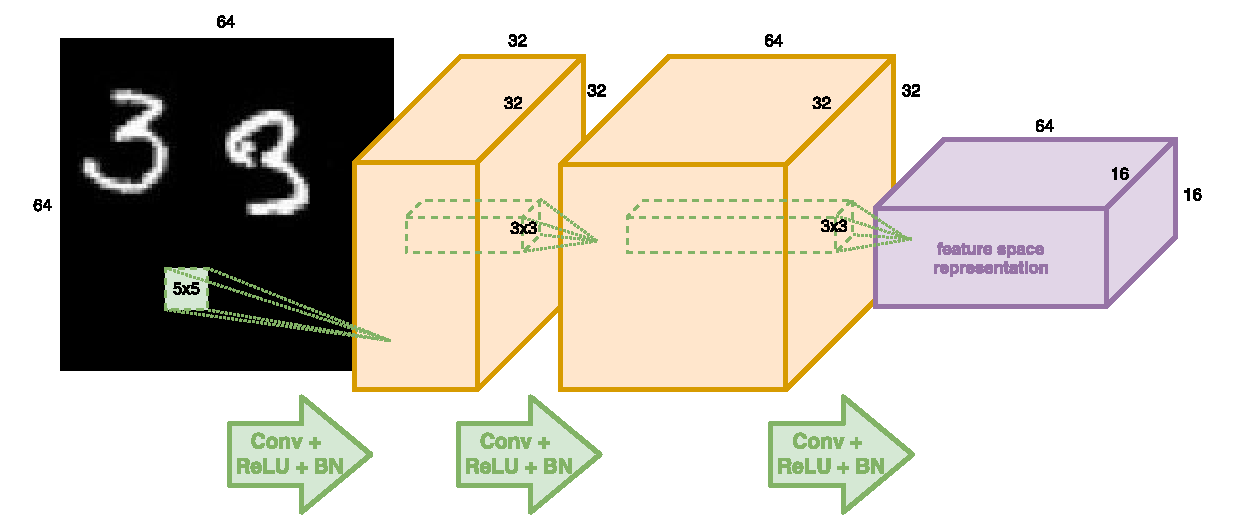
\includegraphics[width=0.9\linewidth]{figures/comp_spatial_encoder.pdf} 
	\caption[Spatial Encoder Component]{Spatial encoding network that maps each input image to its feature space representation (purple) using convolutional layers with ReLU activations and subsequent batch normalizations (green). Intermediate tensors (yellow) are denoted with their height, width and depth.} \label{fig:comp-spatial_encoder}
\end{figure}

No max pooling layers are used because rotation tolerance would be counter-productive in context of frame prediction. This kind of downsampling could remove important details that might be required to successfully reconstruct the image. Instead, each frame is downsampled by using a stride of $ s=2 $ in specific convolutional layers with the motivation that the network itself should learn how to perform such a downsampling operation. Additionally, each convolutional layer is activated using ReLUs and followed by a batch normalization layer to compensate the internal covariate shift of such a deep network model. The resulting frame percepts exhibit a shape of $16\times16\times64$.

\subsubsection{Spatio-Temporal Encoder}



After each percept tensor has been produced by the spatial encoder CNN, it then flows unchanged into a recurrent network to preserve sequential correlations and to learn temporal dynamics. To be more precise, ConvLSTM cells are used to retain the spatial structure of the three-dimensional input data. The cell state $C^{(0)}$ and hidden state $h^{(0)}$ of the spatio-temporal encoder network are initialized with zero by default. Moreover, all convolutional layers within the ConvLSTM cells adapt their number of produced features maps according to the input's depth in order to keep all shape sizes constant. After the whole input sequence of about ten frames has been processed, the resulting cell and hidden states of the last unit then encode the learned motion of the sequence. This representation is then transferred to the following prediction component. It should be noted that the hidden outputs of the encoder's ConvLSTM cells are discarted and not used in the subsequent decoding network. The spatio-temporal encoder component is shown in Figure \ref{fig:comp-spatiotemp_encoder}.

\begin{figure}[htb]
	\centering
	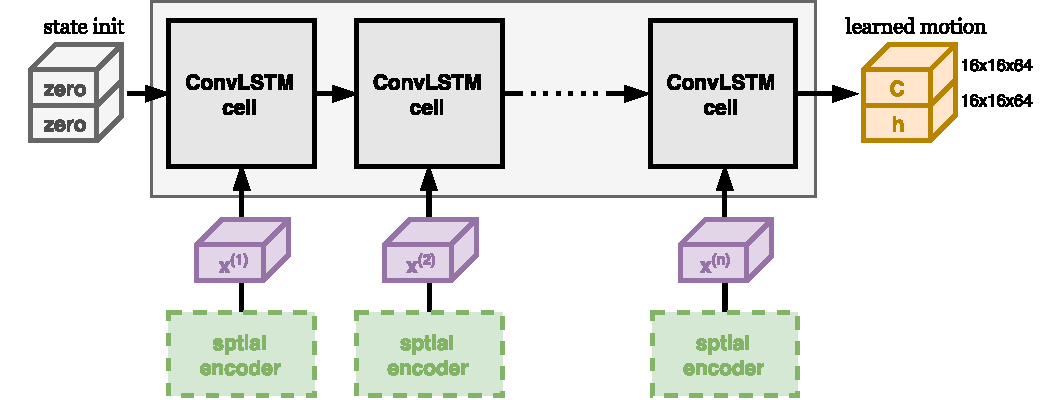
\includegraphics[width=0.9\linewidth]{figures/comp_spatiotemp_encoder.pdf} 
	\caption[Spatio-Temporal Encoding Component]{Spatio-temporal encoder network that encodes a motion representation (orange) based on a frame sequence in feature space (purple). The feature space representations are mapped from each single frame in image space and are produced by the previously described spatial encoder (green).} \label{fig:comp-spatiotemp_encoder}
\end{figure}

\subsubsection{Spatio-Temporal Predictor}

Initialized by the last cell and hidden state of the previous ConvLSTM encoder, the recurrent predictor component takes over to map each frame in feature space at time step $\tau$ to its future representation at time step $\tau + 1$. The spatio-temporal decoder takes advantage of the ConvLSTM cells once more, but it handles the inputs and outputs of each cell in a different way.

\begin{figure}[htb]
	\centering
	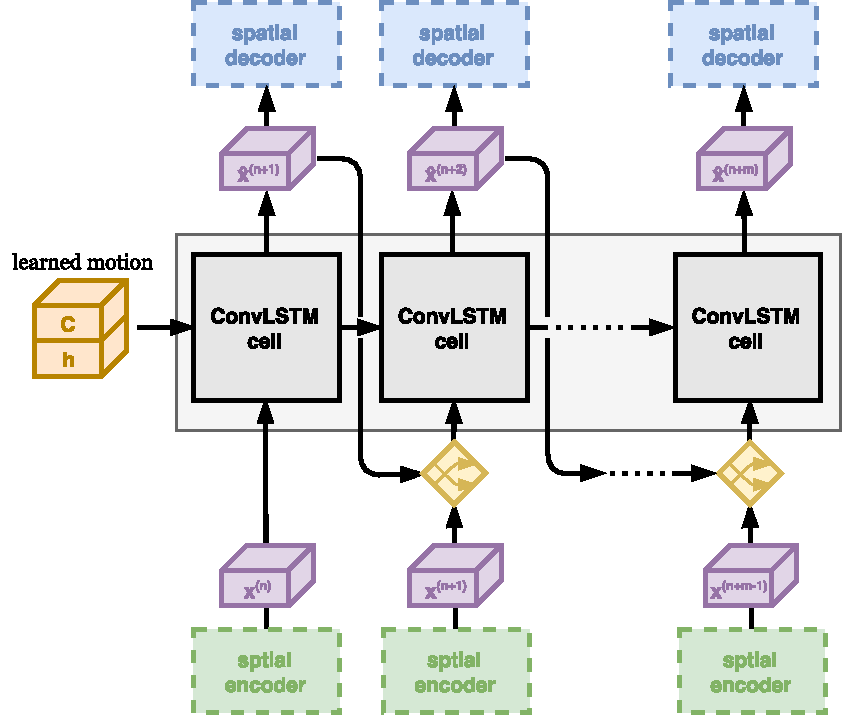
\includegraphics[width=0.8\linewidth]{figures/comp_spatiotemp_decoder.pdf} 
	\caption[Spatio-Temporal Predictor Component]{Spatio-temporal decoding network that maps a frame in future space to its future representation. The ConvLSTM is initialized with the learned motion representation (orange) produced by the recurrent encoder. Each ConvLSTM cell receives either the ground truth representation or the output of the previous cell as its input while training. This decision is made by scheduled sampling components (yellow) at each time step.} \label{fig:comp-spatiotemp_predictor}
\end{figure}

As depicted in Figure \ref{fig:comp-spatiotemp_predictor}, the prediction component utilizes the scheduled sampling technique, earlier presented in Section \ref{sec:sched_sample}, to improve the training performance. By default, the network begins to condition on ground truth frame representations in feature space that have been produced by the spatial encoder component. By decaying the probability of conditioning on the ground truth using an inverse sigmoid function with $\alpha = 1000$, the predictor RNN slowly starts to condition on previously generated frames like in inference mode. With this setting, it takes about \num{10000} training steps until this component predicts future frame representations entirely based on generated outputs. After the entire output sequence has been generated, each single tensor still exhibits a shape of size $16\times16\times64$ and altogether represent the video's future in feature space.

\subsubsection{Spatial Decoder}

To map each frame representation back to the image space, a second CNN is modelled that performs the same transformation steps of the spatial encoder but in reverse order. It therefore uses transposed convolutional layers with rectifier units and batch normalization layers in-between. However, the activation function of the output layer is either a sigmoid or a hyperbolic tangent function to ensure that the generated frames exhibit a valid scale of values. The described spatial decoder is illustrated in Figure \ref{fig:comp-spatial_decoder}.

\begin{figure}[htb]
	\centering
	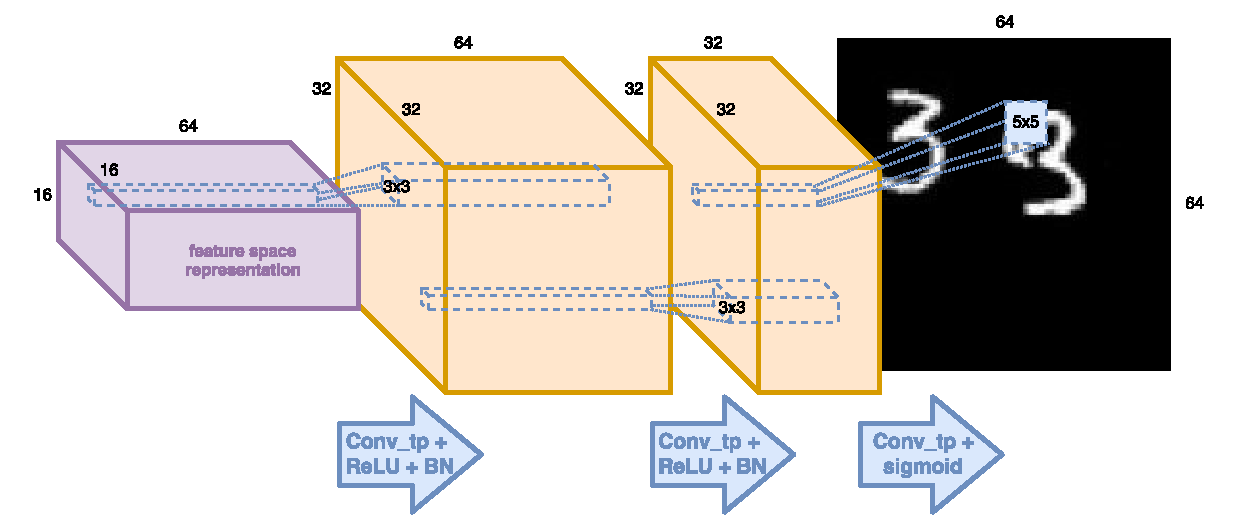
\includegraphics[width=0.9\linewidth]{figures/comp_spatial_decoder.pdf} 
	\caption[Spatial Decoder Component]{Spatial decoding network, which learns to reverse the mapping of the spatial decoder using transposed convolutional layers (blue), to map a feature space representation back to original image space.} \label{fig:comp-spatial_decoder}
\end{figure}


\subsubsection{Loss Layer}

The last component which has to be mentioned is the loss layer used while training the model. Since previous works have shown the problems of using standard loss functions like $\ell_2$ in image processing tasks, as earlier described in Section \ref{sec:perc-loss}, the main objective $\mathcal{L}_{\textrm{main}}$ used in this work is extended by two perceptual motivated bias terms that respect the human notion of visual similarity. The main loss function itself is a placeholder for any commonly used loss function. Depending on the data characteristics, we therefore use $\mathcal{L}_{\textrm{bce}}$, $\mathcal{L}_{\textrm{mse}}$ or $\mathcal{L}_{\textrm{mae}}$ in our context. To counteract the lack of sharpness in predicted frames, a GDL objective function is used as a first extension in order to quantify the sharpness of the image. As a second extension, the SSIM-based loss function is used to assess the image's luminance, contrast and structure. The SSIM-kernel size is chosen to be $k=5$, reasoned by the fact that small image patches are used during the training process only, as well as to improve computational efficiency. The same reasons have also led to the decision to not use the MS-SSIM index. Moreover, RGB image patches are temporarily converted to grayscale which is required to calculate the structural similarity index. Combining these three loss terms together with different weights results in the \textit{triplet loss function} that is used within our experiments:

\begin{equation} \label{eq:triplet}
\mathcal{L}_{\textrm{triplet}}(\textbf{X}, \hat{\textbf{X}}) = \lambda_{\textrm{main}} \mathcal{L}_{\textrm{main}}(\textbf{X}, \hat{\textbf{X}}) + \lambda_{\textrm{gdl}} \mathcal{L}_{\textrm{gdl}}(\textbf{X}, \hat{\textbf{X}}) + \lambda_{\textrm{ssim}} \mathcal{L}_{\textrm{ssim}}(\textbf{X}, \hat{\textbf{X}}) ,
\end{equation}

where $ \textbf{X} $ denotes the ground truth target sequence and $ \hat{\textbf{X}} $ the network's predicted future sequence. The weight and bias parameters of each loss function are neglected for the benefit of simplicity. The coefficients $\lambda_{\textrm{main}}$, $\lambda_{\textrm{gdl}}$ and $\lambda_{\textrm{ssim}}$ control the relative importance of each component in the triplet loss function. A simple default setting is to weight them equally by setting $\lambda_{\textrm{main}} = \lambda_{\textrm{gdl}} = \lambda_{\textrm{ssim}} = 1$.

Additionally, experiments similar to \parencite{gen_img_perc_sim} have been performed where a further loss has been injected to quantify the similarity of feature space representations. Unfortunately, we could not improve our results with such an additional term, because it is not trivial to find an appropriate coefficient $\lambda_{\textrm{feat}}$ to weight this feature space loss relative to other image space losses. On the one hand, it has no visible effect when the coefficient is chosen too low. On the other hand, the accuracy of the predictions decreases tremendously when the coefficient is chosen too high. Due to the difficulties in finding a good balance, as well in the interest of time, such a feature space loss is not used in the final model.


\subsection{Model}

For a better overview regarding the resulting model complexity, Table \ref{tab:model_params} lists the number of trainable parameters for each network component described previously.

\begin{table}[htpb]
  \small
  \centering
  \begin{tabular}{l r}
    \toprule
      \textbf{Component} & \textbf{Trainable parameters} \\
    \midrule
      Spatial encoder \scriptsize{(CNN)} & \num{56416} \\
      Spatio-temporal encoder \scriptsize{(ConvLSTM)} & \num{864512} \\
      Spatio-temporal decoder \scriptsize{(ConvLSTM)} & \num{864512} \\
      Spatial decoder \scriptsize{(CNN)} & \num{56353} \\
    \midrule
    \midrule
      \textbf{Total} & \textbf{\num{1841793}} \\
    \bottomrule
  \end{tabular}
  \caption[Model Parameters]{Overview of the network parameters per component in the described vanilla setting using 1-layer ConvLSTMs.}\label{tab:model_params}
\end{table}

To see everything at a glance, each component is put together in Figure \ref{fig:total_model} to demonstrate the entire model. It has to be noted that not every depicted building block or connection is used when a future sequence is predicted within an inference step. For example, only half as many frames have to be processes by the spatial encoder, because the feature representations of the ground truth target sequence are obviously not available when an actual future prediction is performed. The same is also true for the scheduled sampling components and the loss layer that are only required to train the model. Additionally, the data tensors of each single frame is processed by a separate CNN. Therefore, the trainable parameters in each convolutional layer of the spatial encoder and decoder has to be shared across the whole input sequence. 

Since the overall architecture follows the concept of an encoder-decoder network, it should be argued why this model is likely to learn useful features. According to the argumentation in \parencite[p. 3f.]{unsup_learn_lstm}, it is unlikely to learn the trivial function for the following two reasons. First, an entire sequence of variable size as well as the temporal dynamics have to be encoded and decoded using a fixed-sized representation. In order to accurately predict future frames multiple time steps ahead, the decoder network really has to come up with a learned representation that can distinguish several foreground objects from static background, as well as understand the motion of object and the environmental constraints within a given video scene. Second, the learned motion pattern has to generalize well so that it can be applied to any time step of the sequence. Performing a simple copy of the last state might be almost sufficient when a single frame is predicted only, but not when it has to look further into the future.

\begin{figure}[p]
	\centering
	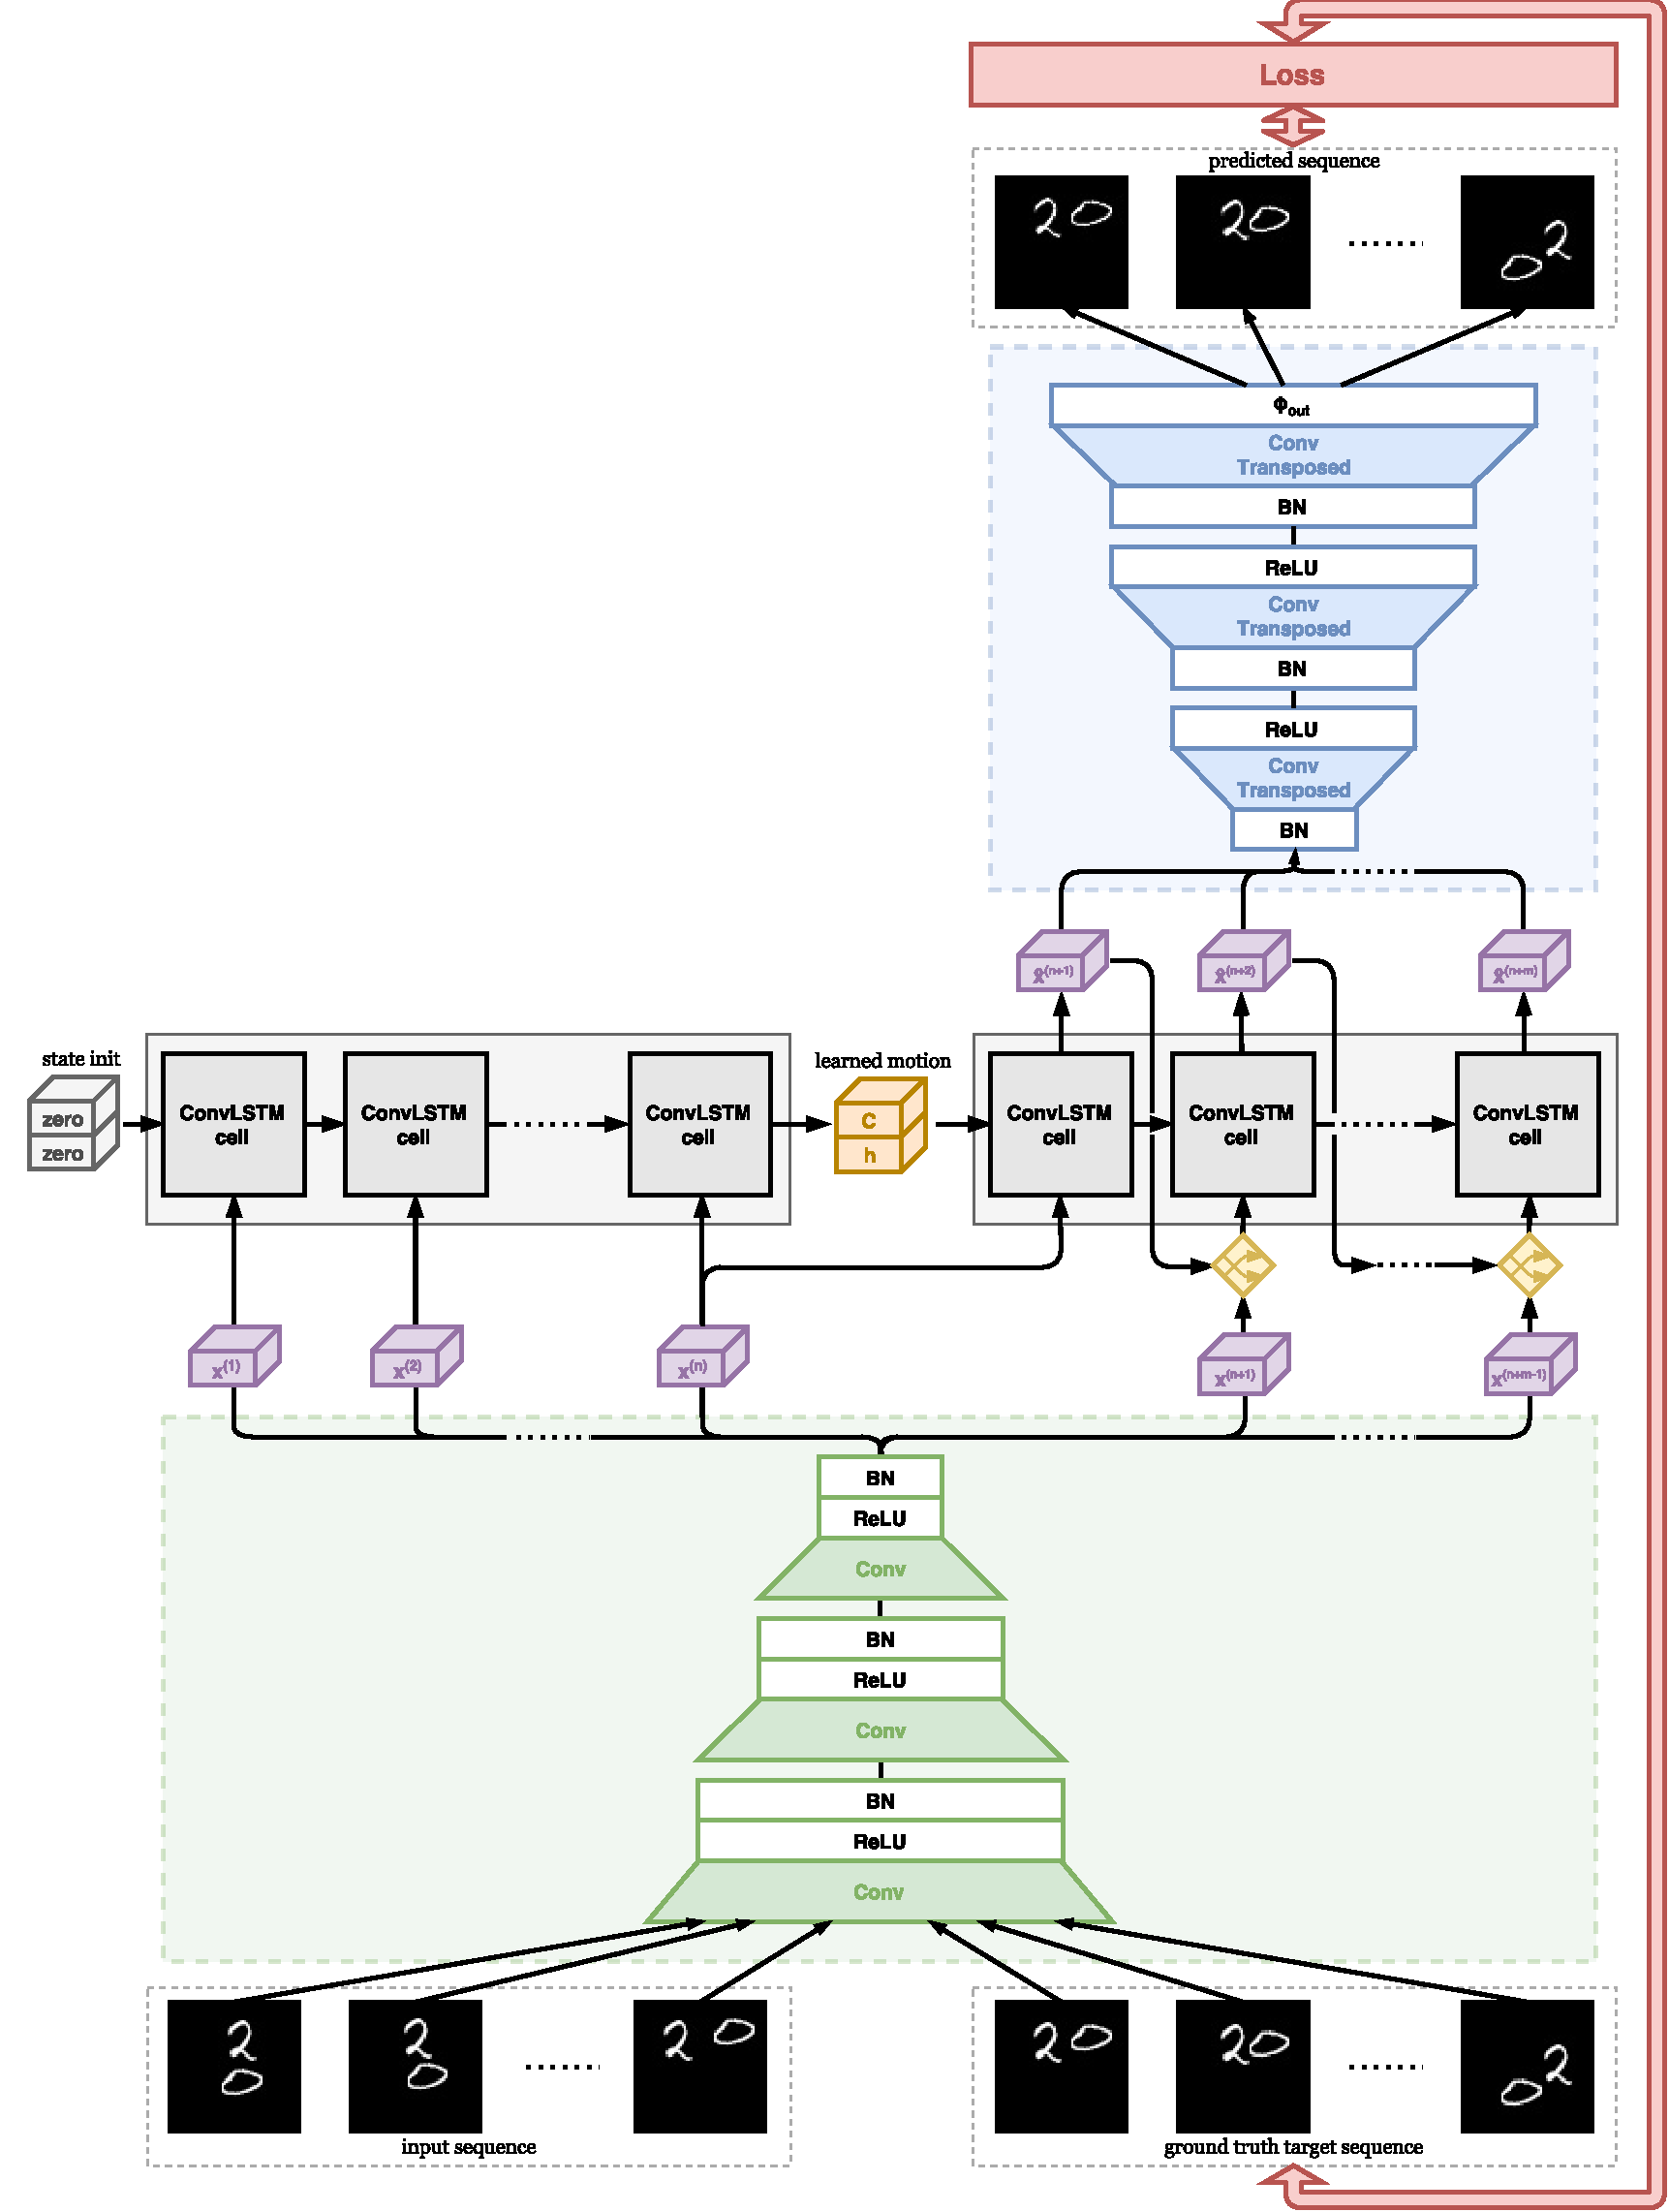
\includegraphics[width=0.96\linewidth]{figures/total_model.pdf}
	\caption[ConvLSTM Encoder-Predictor Model]{The ConvLSTM Encoder-Predictor Model. Weights of the convolutional encoder (green) and decoder (blue) are shared layer-wise across the whole sequence. Spatial encodings of the ground truth frames, scheduled sampling components (yellow) and the loss layer (red) are only used while training.} \label{fig:total_model}
\end{figure}
